
% -----------------------------------------------
% The preamble that follows can be ignored. Go on
% down to the section that says "START HERE" 
% -----------------------------------------------


%%%%%%%%%%%%%%%%%%%%%%%%%%%%%%%%%%%%%%%%%%%%%%%%%%%%%%%%%%%%%%%%%%%%%%%%%%%%%%%%%%%%%%%%%%%%%%%%%%% 

% -----------------------------------------------
% The preamble that follows can be ignored. Go on
% down to the section that says "START HERE" 
% -----------------------------------------------


%Document style
\documentclass[11pt]{article}
\usepackage[margin=1in]{geometry} 
\usepackage{fancyhdr}
\pagestyle{fancy}
\fancyhf{}
\setlength{\headheight}{26pt} 
\fancyhead[l]{Numpty Dumpty\\California Institute of Technology}
\cfoot{\thepage \hspace{1pt} of \pageref{LastPage}}

%Packages in use
\usepackage{
	amsmath,
	amsthm,
	amssymb,
	mathrsfs,
	MnSymbol,
	empheq,
	graphics,
	graphicx,
	enumitem,
	bbm,
	xcolor,
	tikz,
	relsize,
	float,
	verbatim,
	hyperref,
	color,
	courier,
	listings,
	datetime,
	lastpage,
	cite,
	titling,
	caption,
	subcaption}

%\usepackage[strings]{underscore} %does this help with typing underscores?
%\usepackage{mathrsfs}
%\usepackage{palatino}
%\usepackage{enumitem} %alternate enuermating package [(a)]
\usepackage[english]{babel}
\usepackage[utf8]{inputenc}
\usepackage[T1]{fontenc}
\usepackage[framemethod=default]{mdframed}
\usepackage[super]{nth}
%\graphicspath{{../latexfigs/}} %specifies graphicspath

\mdfdefinestyle{MyFrame}{%
	linecolor=black,
	outerlinewidth=5pt,
	%roundcorner=20pt,
	innertopmargin=5pt,
	innerbottommargin=5pt,
	innerrightmargin=5pt,
	innerleftmargin=5pt,
	leftmargin = 5pt,
	rightmargin = 5pt
	%backgroundcolor=gray!50!white}
}

\renewcommand{\maketitlehooka}{\begin{mdframed}[style=MyFrame]}
\renewcommand{\maketitlehookd}{\end{mdframed}\vspace{5 mm}}





%Hyperlink Setup
\hypersetup{
	colorlinks,
	citecolor=black,
	filecolor=black,
	linkcolor=black,
	urlcolor=blue
}


\newenvironment{theorem}[2][Theorem]{\begin{trivlist}
\item[\hskip \labelsep {\bfseries #1}\hskip \labelsep {\bfseries #2.}]}{\end{trivlist}}
\newenvironment{lemma}[2][Lemma]{\begin{trivlist}
\item[\hskip \labelsep {\bfseries #1}\hskip \labelsep {\bfseries #2.}]}{\end{trivlist}}
\newenvironment{exercise}[2][Exercise]{\begin{trivlist}
\item[\hskip \labelsep {\bfseries #1}\hskip \labelsep {\bfseries #2.}]}{\end{trivlist}}
\newenvironment{problem}[2][Problem]{\begin{trivlist}
\item[\hskip \labelsep {\bfseries #1}\hskip \labelsep {\bfseries #2.}]}{\end{trivlist}}
\newenvironment{question}[2][Question]{\begin{trivlist}
\item[\hskip \labelsep {\bfseries #1}\hskip \labelsep {\bfseries #2.}]}{\end{trivlist}}
\newenvironment{corollary}[2][Corollary]{\begin{trivlist}
\item[\hskip \labelsep {\bfseries #1}\hskip \labelsep {\bfseries #2.}]}{\end{trivlist}}
\newenvironment{solution}{\begin{proof}[Solution]}{\end{proof}}


%%%%%%%%%%%%%%%%%%%%%%%%%%%%%%%%%%%%%%%%%%%%%%%%%START_MATLAB%%%%%%%%%%%%%%%%%%%%%%%%%%%%%%%%%%%%%%%%%%%%%%%%%%%%%%%%%%%

\definecolor{mygreen}{RGB}{28,172,0} % color values Red, Green, Blue
\definecolor{mylilas}{RGB}{170,55,241}

\lstset{language=Matlab,%
	basicstyle=\small\ttfamily, %or \small or \footnotesize etc.
	breaklines=true,%
	morekeywords={matlab2tikz},
	keywordstyle=\color{blue},%
	morekeywords=[2]{1}, keywordstyle=[2]{\color{black}},
	identifierstyle=\color{black},%
	stringstyle=\color{mylilas},
	commentstyle=\color{mygreen},%
	showstringspaces=false,%without this there will be a symbol in the places where there is a space
	numbers=left,%
	numberstyle={\tiny \color{black}},% size of the numbers
	numbersep=9pt, % this defines how far the numbers are from the text
	emph=[1]{for,end,break},emphstyle=[1]\color{red}, %some words to emphasise
	%emph=[2]{word1,word2}, emphstyle=[2]{style},    
}
%%%%%%%%%%%%%%%%%%%%%%%%%%%%%%%%%%%%%%%%%%%&&%%%%%%END_MATALB%%%%%%%%%%%%%%%%%%%%%%%%%%%%%%%%%%%%%%%%%%%%%%%%%%%%%%%%%%%



\setlength\parindent{0pt} %sets noindent for entire file




%My shortcuts
\newcommand{\N}{\mathbb{N}}
\newcommand{\Z}{\mathbb{Z}}
\newcommand{\R}{\mathbb{R}}
\newcommand{\C}{\mathbb{C}}
\newcommand{\E}{\mathbb{E}}
\newcommand{\Pro}{\mathbb{P}}
\newcommand{\Lag}{\mathscr{L}}
\newcommand{\lm}{\lambda}
\newcommand{\limn}{\lim_{n \rightarrow \infty}}
\newcommand{\limN}{\lim_{N \rightarrow \infty}}
\newcommand{\Rn}{\mathbb{R}^n}
\newcommand{\sn}{\mathbb{S}^n}
\newcommand{\1}{\mathbbm{1}}
\newcommand{\ata}{A^TA}
\newcommand{\Rmn}{\mathbb{R}^{m \times n}}
\newcommand{\Rnn}{\mathbb{R}^{n \times n}}
\newcommand{\Rnm}{\mathbb{R}^{n \times m}}
\newcommand{\Var}{\operatorname{Var}}
\newcommand{\Cov}{\operatorname{Cov}}
\newcommand{\Bias}{\operatorname{Bias}}
\newcommand{\ba}{\[\begin{aligned}}
\newcommand{\ea}{\end{aligned}\]}







\title{CMS 155 Miniproject 1 Report} 
\author{Lucien Werner\\Spencer Gordon} 

% \pagestyle{fancy}
\fancyhead[r]{CMS/CS/EE 155\\Machine Learning \& Data Mining}




\begin{document}


% ------------------------------------------ %
% MAKE TITLE                 %
% ------------------------------------------ %
\thispagestyle{empty} %keep first page plain
\maketitle

% ------------------------------------------ %
% START HERE                 %
% ------------------------------------------ %


\section{Introduction}
\medskip
\begin{itemize}
  
\item \textbf{Group Members:} Lucien Werner and Spencer Gordon
  
\item \textbf{Team name:} Numpty Dumpy (\nth{11} place)
  
\item \textbf{Division of labour} \\
  Although we mostly did pair coding, the table below displays a rough division of tasks. 
  \begin{table}[h]
    \centering
    \begin{tabular}{l|l}
      Task                                   & Person   \\ 
      \hline
      Regression \& ensemble methods coding~ & Lucien  \\
      Neural net coding                      & Spencer  \\
      Report writing                         & Shared  
    \end{tabular}
  \end{table}
  
\item \textbf{List of files in submission}
  \begin{itemize}
  \item \texttt{regression.py}	
  \item \texttt{adaboost.py}	
  \item \texttt{gradientboosting.py}	
  \item \texttt{randomforest.py}	
  \item \texttt{naivebayes.py}
  \item \texttt{deepnet.ipynb}	
    
    
    
    
  \end{itemize}
\item \textbf{GitHub repository:} \url{https://github.com/sgord512/cs155_miniproject1}
\end{itemize}



\section{Overview}
\medskip
\begin{itemize}
  
\item \textbf{Models and techniques tried}\\
  
  We tried a range of machine learning models and used a subset of the given training data to validate and compare their performance. For each model class we tried, we tuned our model hyperparameters by doing a grid search across a space of hyperparameters and using cross-validation. We tried simpler models (e.g., logistic regression) first and progressed to more sophisticated models (e.g., ensemble methods and neural nets). We avoided the temptation to overfit the model to the training data and the public leaderboard, because we thought doing so might ultimately penalize us on the private leaderboard. The sparse, high-dimensional character of our data encouraged us to experiment heavily with linear models which are well suited to such datasets and avoid support vector classifiers (SVCs) which would have been infeasible to train on such a large dataset. We also experimented with decision tree classifiers (and ensembles of them) because they are quick to train and relatively robust. Ultimately these did not prove to give the performance we sought. Neural nets were our last resort due to the difficulty in finding an optimal structure in a systematic way. To our surprise thought, this model gave incrementally better performance for us on both the public and private leaderboard than our linear models. 
  
\item \textbf{Work timeline}
  \begin{itemize}
  \item \textbf{February 2-4:} Logistic regression
  \item \textbf{February 5-7} Ensemble methods 
  \item \textbf{February 8:} Neural net
  \end{itemize}
  
\end{itemize}


\section{Approach}
\medskip
\begin{itemize}
  
\item \textbf{Data processing and manipulation:} We tried several methods to normalize the training data:
  \begin{itemize}
  \item TF-IDF transformation (discounts words that appear frequently in other reviews)
  \item Logarithmic normalization ($X_i=\log(1+X_i)$) (discounts higher word counts)
  \item Binary normalization (converts all non-zero entries to 1)
  \item Point-wise normalization (divides every feature in a datapoint by the norm of the entire datapoint).
  \end{itemize}
  None of these normalization procedures improved the accuracy of our classifier, although in some cases (TF-IDF, for example) there was a significant increase in the training speed. The trade-off between accuracy and training speed was not universal across the models we tested, but we ultimately decided against normalization for our neural network.
\item \textbf{Details of models and techniques:} We tried the following models:
  \begin{itemize}
  \item \textbf{Logistic Regression:} Linear regression with logistic loss and regularization strength $C=0.1$ was the first thing we tried, and ultimately it gave better performance than anything besides the neural net. Fitting this model was primarily about finding the best regularization strength. Using \texttt{sklearn}'s \texttt{GridSearchCV} method, we set a range of parameters for regularization strength, solver, and max iterations to train the model over. To asses the performance of the different parameter sets, we used 5-fold cross validation of the training set. Bag-of-words data is high dimensional and sparse, indicating that some kind of regression was a good place to start the modeling. 
  \item \textbf{Random Forest:} Random forest classifiers are good all-purpose models and if the weak classifiers are shallow enough, they train quickly as well. We tested performance using \texttt{sklearn}'s \texttt{RandomizedSearchCV} method across a range of parameters including the number of weak classifiers, min\_sample\_split, and max\_tree\_depth. 
  \item \textbf{Gradient Boosting and AdaBoost:} Gradient boosting and AdaBoost (using \texttt{sklearn}'s \texttt{GradientBoostingClassifier} and \texttt{AdaBoostClassifier}, respectively) with shallow decision trees as weak classifiers did not give better results than the random forest. After tuning the hyperparameters with randomized grid search over a subset of the parameter space, we only achieved accuracy in the low 80\% on our validation dataset. 
  \item \textbf{Naive Bayesian Classifier:} We used \texttt{sklearn}'s \texttt{GaussianNB} classifier. Bayes classifiers generally train quickly on high dimensional data. We found this to be the case but the accuracy was poor. 
  \item \textbf{Neural Network:} We used \texttt{Keras} for all of our neural network models. We used a 3-layer neural network with up to 1300 hidden units, ReLU activation, and Dropout layers between all of the hidden layers. We tuned the dropout probability of all the layers using the approach from the \nth{4} homework. This method ended up performing marginally better on our validation dataset and significantly better on the public leaderboard. See Figure \ref{acc_vs_dropout_prob} for an illustration of the average accuracy (computed through 5-fold cross validation) for one of the models we tried. This model had 3 layers of hidden units, with 250, 100, and 50 units in order from the input layer to the output layer, each of which was followed by a ReLU activation layer and a dropout layer. 
    \begin{figure}[h]
      \centering
      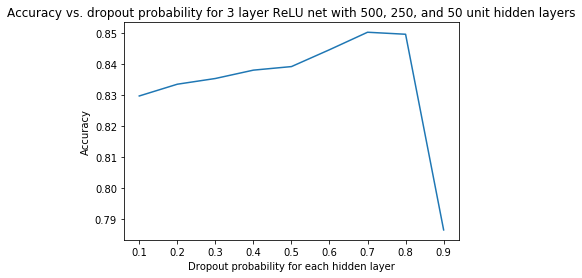
\includegraphics[scale=0.7]{accuracy_vs_dropout_prob.png}
      \caption{Illustration of accuracy vs dropout probability for one neural net architecture we tried. We were surprised by how high we the dropout probability could go before accuracy started to decrease.}\label{acc_vs_dropout_prob}
    \end{figure}
    After trying this model, we experimented with increasing the number of hidden units in some of the layers, and found that we had better performance when increasing the number of units in the first layer to 1000. Our most successful submission was the resulting architecture trained as follows: We trained the network for 20 epochs with a batch size of 64, using the \texttt{rmsprop} optimizer and \texttt{binary\_crossentropy} as our loss function. 

    After finding this very successful model, we tried the \texttt{adam} optimizer, and found that this gave worse performance. We also tried increasing the number of epochs of training, but found that this caused accuracy to decrease, suggesting that the model was overfitting. We also tried implementing early stopping, training until the accuracy on our small validation set began to increase but this also failed to increase accuracy, since the accuracy from one epoch to the next would often decrease, and so early stopping with no lower limit on epochs trained resulted in too few epochs of training; on the other hand, we tried training for 20 epochs and then continuing to train until accuracy decreased, but this resulted in no more than 25 epochs of training and slightly worse accuracy on the public test set. We were less systematic about hyperparameter optimization at this point due to time constraints. If we were to have more time we would probably do a grid search over various neural net architectures, varying the number of hidden units in each layer, the optimizer, the number of epochs, and the batch size, as well as the dropout probabilities of each layer. 
  \end{itemize}

\end{itemize}


\section{Model Selection}
\medskip
\begin{itemize}
  
\item \textbf{Scoring} 
  We used accuracy as our scoring metric in all tests. It is defined as
  $$
  \text{accuracy}=\frac{\text{\# of matches}}{\text{\# of datapoints}}.
  $$
  When training with cross-validation, accuracy scores were averaged across folds. Our initial experiments with logistic regression set a baseline $\sim 84$\% accuracy. For example, see Fig. \ref{acc} for an example of parameter vs. accuracy plot. In this case we were seeking the optimal regularization strength $C$ for a simple logistic regression model. Each of our models was validated this way in order to determine the highest performing parameters
    
\item \textbf{Validation and Test} 
  We set aside 5\% (1000 datapoints) of the training set for a fixed random seed to validate our models, separate from in-sample cross-validation during training. Scores from this validation step generally tracked closely to those subsequently attained on the public leaderboard.
    \begin{figure}[h]
  	\centering
  	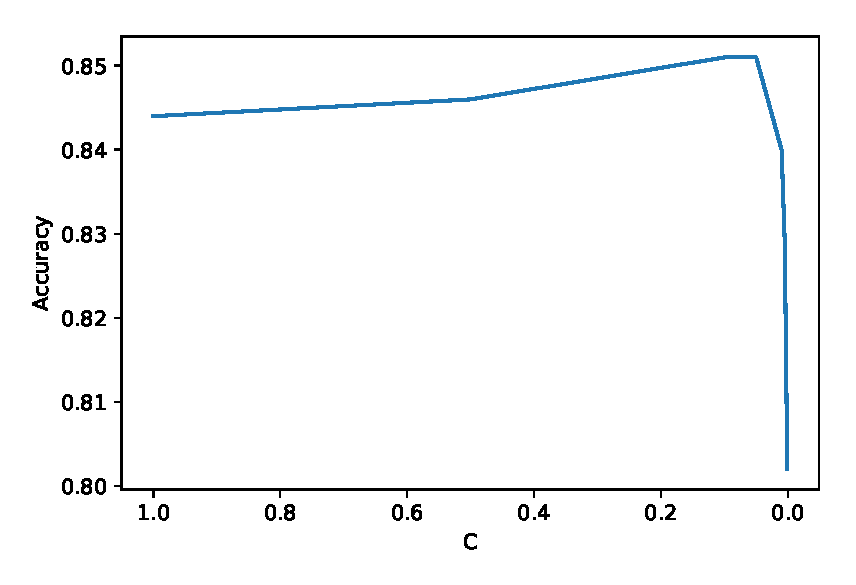
\includegraphics[width=0.7\textwidth]{acc.eps}
  	\caption{Regularization strength $C$ vs. model accuracy for Logistic Regression}\label{acc}
  \end{figure}
\end{itemize}



\section{Conclusion}
\medskip
\begin{itemize}
  
\item \textbf{Discoveries} 
  We discovered that despite trying and optimizing numerous regression models, model ensembles, and hyperparameters, a neural network still gave the (marginally) best performance. It was also surprising that simple logistic regression performed nearly as well on this dataset. Another crucial point was that tuning hyperparameters was \textit{the} crucial aspect of achieving good classification performance. In hw and lecture, this is not something we had to work with too much, especially w.r.t. the preferred amount of regularization. 
  
\item \textbf{Challenges} 
  Avoiding overfitting to the public leaderboard was on our mind as we validated the models. By setting aside 5\% of our training set to validate our model accuracy after training, we had a point of reference for the leaderboard score. Otherwise, establishing the neural net architecture was a process that felt like a lot of trial and error. Given the number of possible structures and parameter values that are available to a neural net, it seemed like we might have landed upon something that worked well partially by luck. Doing this again, we would spend more time systematically testing different model structures (number of layers, activation functions, number of units per hidden layer, etc.), or alternatively considering ensembles of shallow neural nets. 
  
\item \textbf{Concluding Remarks} 
  An interesting feature of this project was that there seemed to be a fundamental limit on the performance of machine-learned models on this dataset. The scoreboard results were all clustered within a couple percentage points around 85\%. We found that most models we tried would approach this ceiling after tuning hyperparameters; in other words, the learning limit of the data seemed to be model independent. (Note that this clustering does not prove anything about the existence of such a limit though.)
  
\end{itemize}






%%%%%%%%%%%%%%%%%%%%%%%%%%%%%%%%%%% START_BIBLIOGRAPHY%%%%%%%%%%%%%%%%%%%%%%%%%%%%%%%%%
\medskip
\nocite*
\bibliographystyle{unsrt}
\bibliography{biblio}
%%%%%%%%%%%%%%%%%%%%%%%%%%%%%%%%%%%% END_BIBLIOGRAPHY%%%%%%%%%%%%%%%%%%%%%%%%%%%%%%%%%%


%%%%%%%%%%%%%%%%%%%%%%%%%%%%%%%%%%%%%% START_CODE%%%%%%%%%%%%%%%%%%%%%%%%%%%%%%%%%%%%%%
\begin{comment}
  
  
  \clearpage
  \section*{Appendix: Python Code}

  \subsection*{Problem 2}
  \lstinputlisting[language=Python]{p2.py}

\end{comment}

%%%%%%%%%%%%%%%%%%%%%%%%%%%%%%%%%%%%%%%% END CODE%%%%%%%%%%%%%%%%%%%%%%%%%%%%%%%%%%%%%%



\end{document}


% -----------------------------------------------
% Ignore everything that appears below this.
% -----------------------------------------------





%%%%%%%% Old Material

% %% BEGIN BIBLIOGRAPHY++++++++++++++++++++++++++++++++++++++++++++++++++++++++++++++%%

% \newpage
% \begin{thebibliography}{9}


% \bibitem{andrewlewis} 
%   Website of Professor Andrew D. Lewis, Department of Mathematics & Statistics at Queen's University 
%   \\\texttt{http://www.mast.queensu.ca/\~andrew/erdos.shtml}


% \bibitem{adam} 
%   Website of Professor Adam Wierman, Erd\H{o}s Number
%   \\\texttt{http://users.cms.caltech.edu/~adamw/erdosnumber.html}


% \bibitem{erdos} 
%   The Erd\H{o}s Number Project
%   \\\texttt{https://oakland.edu/enp/}


% \bibitem{gscholar} 
%   Google Scholar
%   \\\texttt{https://www.scholar.google.com}

%   \begin{comment}
%   \bibitem{latexcompanion} 
%     Michel Goossens, Frank Mittelbach, and Alexander Samarin. 
%     \textit{The \LaTeX\ Companion}. 
%     Addison-Wesley, Reading, Massachusetts, 1993.

%   \bibitem{einstein} 
%     Albert Einstein. 
%     \textit{Zur Elektrodynamik bewegter K{\"o}rper}. (German) 
%     [\textit{On the electrodynamics of moving bodies}]. 
%     Annalen der Physik, 322(10):891?921, 1905.

%   \end{comment}


% \end{thebibliography}
% %% END BIBLIOGRAPHY++++++++++++++++++++++++++++++++++++++++++++++++++++++++++++++++%%


\begin{figure}[h]
  \centering
  \includegraphics[width=.6\textwidth]{p2b.eps}
  \label{p2b}
  \caption{Decision Tree, Gini, Maximum Tree Depth}
\end{figure}
